\documentclass{article}

\usepackage{listings} % For code formatting
\usepackage[utf8]{inputenc}  % For encoding support
\usepackage{amsmath}         % For mathematical formatting
\usepackage{graphicx}        % For including images
\usepackage{xcolor}
\usepackage[a4paper, left=0.5in, right=0.5in, top=0.5in, bottom=0.5in]{geometry}  % Adjust margins here
\usepackage{tcolorbox}
\usepackage{palatino}  % Use Inconsolata font (or replace with your choice)
\usepackage{amsmath, amssymb, array, booktabs}

% Define colors
\definecolor{codebg}{RGB}{240, 240, 240}  % Light gray background
\definecolor{framecolor}{RGB}{100, 100, 100}  % Dark gray frame
\definecolor{titlebg}{RGB}{30, 30, 30}  % Dark title background
\definecolor{titlefg}{RGB}{255, 255, 255}  % White title text

% Custom lstset
\lstset{
    language=C++,                    
    basicstyle=\ttfamily\footnotesize\fontfamily{zi4}\selectfont, % Use Inconsolata
    keywordstyle=\bfseries\color{blue},        
    commentstyle=\itshape\color{gray},        
    stringstyle=\color{red},          
    numbers=left,                     
    numberstyle=\tiny\color{blue},    
    frame=single,                     
    breaklines=true,                   
    captionpos=b,                      
    backgroundcolor=\color{codebg},  % Light gray background
    rulecolor=\color{framecolor},    % Dark frame
    tabsize=4                         
}

% Custom command to add a styled heading
\newtcbox{\codebox}{colback=titlebg, colframe=titlebg, colupper=titlefg, 
  boxrule=0pt, arc=5pt, left=5pt, right=5pt, top=3pt, bottom=3pt}

\title{AnySeq/GPU: A Novel Approach for Faster Sequence Alignment on GPUs}

\author{Ayush Raina, 22148}
\date{\today}

\begin{document} 

\maketitle

\subsection*{Overview}
The paper introduces \textbf{AnySeq/GPU}, a fast sequence alignment library optimized for GPUs. It improves performance by reducing memory accesses using \textbf{warp shuffles} and \textbf{half precision arithmetic}, and it uses the \textbf{AnyDSL compiler} for efficient GPU code generation. The library achieves up to \textbf{3.8 TCUPS}, outperforming previous GPU-based aligners like GASAL2 and NVBIO by up to \textbf{19.2x}. It runs efficiently on both NVIDIA and AMD GPUs and is open-source.

\subsection*{Motivation}
Sequence alignment is essential in bioinformatics, especially with the rapid growth of \textbf{Next-Generation Sequencing (NGS)} data. Traditional alignment algorithms like \textbf{Needleman-Wunsch} and \textbf{Smith-Waterman} use dynamic programming (DP) and have high time complexity, making them slow for large-scale NGS data (both short and long reads). While many alignment tools have been developed for \textbf{CPUs, GPUs, and FPGAs}, current GPU-based tools often suffer from:
    Inefficient memory access patterns,
    Lack of performance portability across different sequence lengths and alignment types,
    Limited optimization to only specific CUDA-enabled GPUs.
To overcome these limitations, the authors propose AnySeq/GPU, an optimized GPU-based extension of the AnySeq library.

\subsection*{Methodology and Key Contributions}
1. \textbf{Unique Parallelization Strategy: }Introduces a new fine grained GPU Parallelization technique using \textbf{warp intrinsics} and a novel \textbf{DP Matrix Partitioning} scheme that handles batches with varying sequence lengths efficiently. \\ \\ 
2. \textbf{Hardware Independent Implementation: }It leverages \textbf{AnyDSL}, a domain specific language framework which is used to generate optimized kernels for both \textbf{NVIDIA} and \textbf{AMD} GPUs. \\ \\ 
3. \textbf{High Performance: }Achieves over \textbf{80\%} of peak GPU Performance across a range of alignment types with speedups of \textbf{3.6x to 19.2x} compared to existing GPU-based libraries.

\subsection*{Sequence Alignment}
Given two DNA Sequences $Q = (q_1,q_2,...,q_m)$ and $S = (s_1,s_2,...,s_n)$, the goal of sequence alignment is to compute the best match between them using \textbf{Dynamic Programming (DP)}. The DP Matrix $H(i,j)$ stores the optimal alignment score between the $Q(1:i)$ and $S(1:j)$ subsequences and is recursively defined as: 
\begin{equation}
H(i,j) = \max{\begin{cases}
  H(i-1,j-1) + \sigma(q_i,s_j) \\
  H(i-1,j) - \alpha \\
  H(i,j-1) - \alpha \\
\end{cases}}
\end{equation}

\begin{figure}
    \centering
    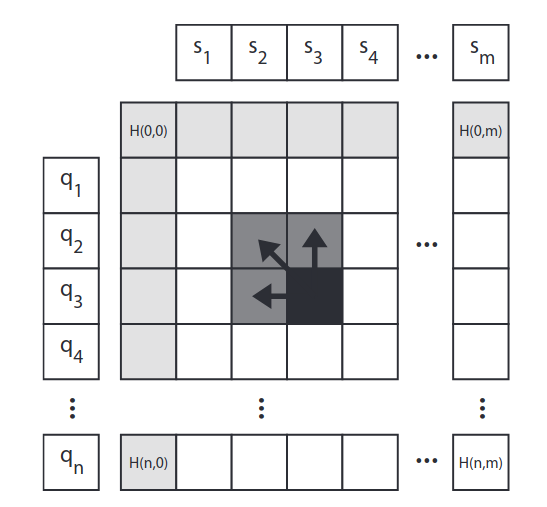
\includegraphics[width=0.2\textwidth]{dpmatrix.png}
    \caption{Dynamic Programming Matrix for Sequence Alignment}
    \label{fig:dp_matrix}
\end{figure}

where $\alpha$ is the constant gap penalty and $\sigma(q_i,s_j)$ is the substitution cost function. The final alignment score is found in $H(m,n)$. In the original paper, other types of gap penalty scheme can be found, but we will consider the constant gap penalty scheme for simplicity.

% \subsection*{Approach}
% The core idea is to compute \textbf{one alignment per warp}, where a warp consists of 32 threads executing in lockstep. All these threads work together to compute the DP matrix. To achieve high efficiency following optimizations are made: \\\\
% 1. \textbf{Warp Shuffles: } All DP matrix values are computed using fast GPU registers, with thread to thread communication handled via \textbf{warp shuffle instructions} which minimizes memory latency. \\
% 2. \textbf{Reduced Memory Traffic: } Sequence characters are loaded once per warp and reused through intra warp shuffles, avoiding redundant loads from memory. \\
% 3. \textbf{Partitioning: }For longer sequences, the DP Matrix is Partitioned, enabling processing in manageable chunks. \\
% 4. \textbf{Optimal Traceback: } The method supports optional traceback in linear space.

\subsection*{Mapping Matrix Cells and Sequences to Threads}
Algorithm assigns each warp (32 threads $T_0,T_1,...,T_{31}$) to compute pairwise alignment between seuqence $Q$ of length m and sequence $S$ of length n. The DP Matrix $\textbf{H} \in \mathbb{R}^{(m+1) \times (n+1)}$ is computed in \textbf{tiles}, where each thread $T_t$ is responsible for computing $k$ columns of $\textbf{H}$ giving the relation $n = kp - 1$. The matrix is filled diagonally over $m+p$ iterations, where in each iteration $i$, thread $T_t$ computes $(i-t)^{th}$ row of its $k$ assigned columns, according to recurrence relation given. \\

To reduce memory traffic, DP values are stored in \textbf{local-thread registers} and are shared across other threads in the warp using \textbf{warp shuffle instructions} to access neighbour's values. This allows for fast intra-warp communication and minimizes the need for global memory accesses.
Subject characters S are loaded once by each thread and used to construct a scoring profile in shared memory. This stores $\sigma(q_i,s_j)$ for all $s_j \in S, q_i \in Q$ and enables efficient lookups. \\

Query characters $Q$, whose values change across rows, are loaded only every $p$ iterations and then propagated between threads using registers and warp shuffles \textbf{(e.g., shfl\_up and shfl\_down)} to avoid global memory loads. Each thread maintains two registers $c_{q0}$ and $c_{q1}$, where $c_{q0}$ stores the current query character $Q_{i-t-1}$ and $c_{q1}$ stores the next query character for the next iteration. Only in the iterations where $i\mod p = 0$, each thread loads a new character $q_{i+t}$ from memory into $c_{q1}$. In all other iterations, threads update $c_{q0}$ and $c_{q1}$ using warp shuffles. 

\subsection*{Handling Long Sequences with Multi Stage Partioning}
In modern GPUs, the number of registers per thread is limited (For NVIDIA, its 255), which restricts the size of $k$ i.e number of columns that each thread is going to process. To support for the longer sequences, the algorithm partitions the DP Matrix into $l$ non overlapping submatrices, each of size: $(m+1) \times (\frac{n+1}{kp})$. These submatrices are computed sequentially from left to right in $l$ stages.At the end of each stage, the rightmost DP values computed by thread $T_{31}$ are stored in shared or global memory and these values are read by $T_0$ in the next stage. To minimize memory access overhead, this \textbf{stage-wise boundary communication} also uses warp shuffles where possible, similar to how query characters are propagated.
\begin{figure}[h]
    \centering
    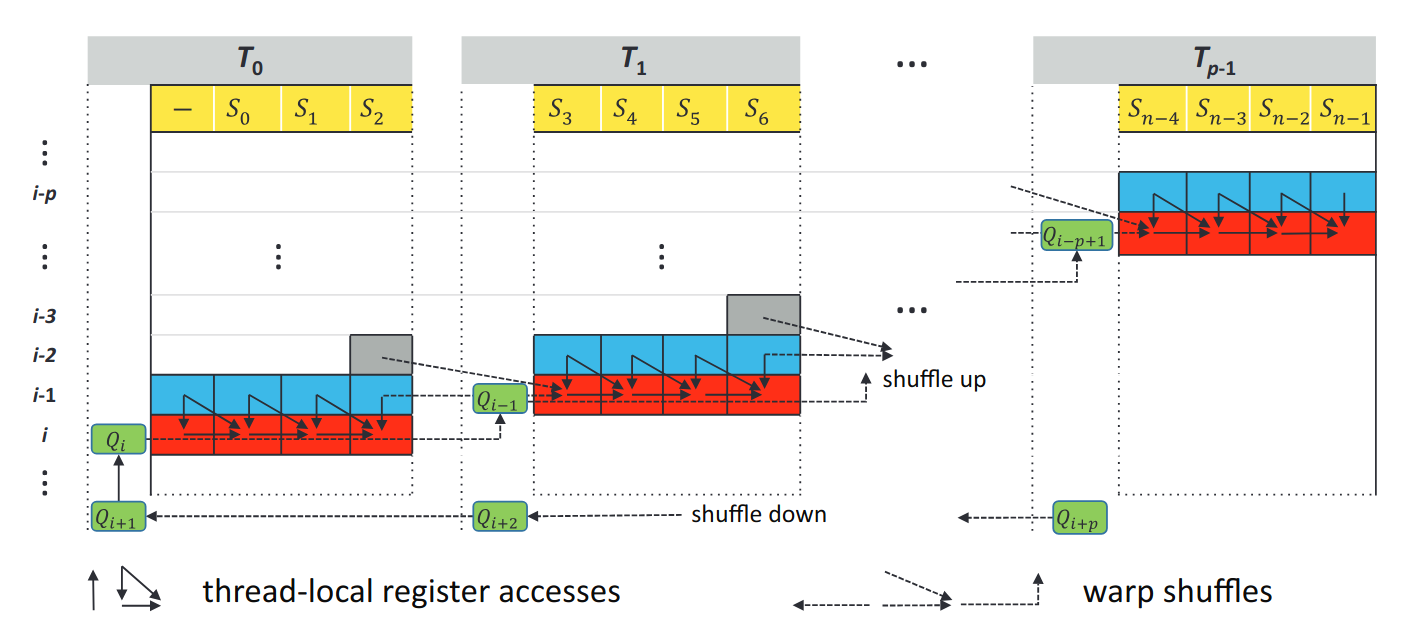
\includegraphics[width=0.6\textwidth]{partition.png}
    \caption{Partitioning of DP Matrix for Long Sequences}
    \label{fig:partitioning}
\end{figure}

\subsection*{Automatic GPU Kernel Generation using AnyDSL}
AnySeq/GPU uses user-guided partial evaluation (PE) within the AnyDSL framework to automatically generate GPU kernels that are specialized for specific alignment types such as local or global alignments, hardware architectures, sequence lengths, and scoring schemes such as linear or affine. This approach enables high performance while avoiding code duplication.
\begin{figure}[h]
    \centering
    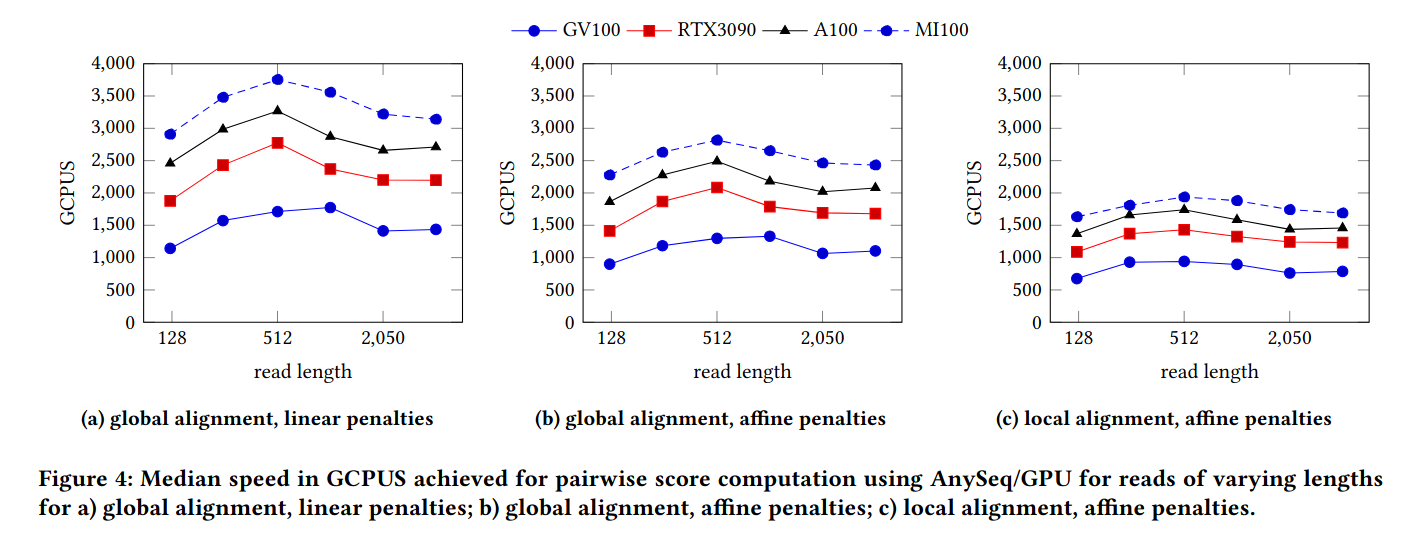
\includegraphics[width=0.65\textwidth]{results1.png}
\end{figure}

Figure 4 reports the median performance in GCUPS (giga cell updates per second) for pairwise alignment using AnySeq/GPU across varying read lengths. Three alignment modes are evaluated:

    (a) Global alignment with linear gap penalties

    (b) Global alignment with affine gap penalties

    (c) Local alignment with affine penalties

For all modes, performance peaks around read length $\sim$ 512, where the throughput reaches up to 3,600 GCUPS on AMD MI100. Linear penalties (panel a) allow simpler recurrences, enabling higher throughput than affine gaps. Among GPUs, MI100 $>$ A100 $>$ RTX 3090 $>$ GV100 in GCUPS, reflecting differences in memory bandwidth and compute power.

\subsection*{Critical Analysis}

\textbf{Strengths:} \\
AnySeq/GPU introduces a warp-level parallelization strategy that leverages GPU registers and warp shuffles for efficient dynamic programming (DP) matrix computation. It supports both short and long reads, achieves high throughput (up to 3.8 TCUPS), and maintains $>$80\% hardware efficiency across different GPUs. Its use of partial evaluation allows architecture-specific optimization while keeping the codebase general and portable. \\ \\
\textbf{Why these contributions matter:} \\
Sequence alignment is a core step in many bioinformatics pipelines, and optimizing it for modern GPU hardware directly translates to faster genome analysis. Unlike earlier tools optimized only for short reads or specific architectures, AnySeq/GPU generalizes across read lengths and GPU vendors. Its in-register design and architecture-agnostic implementation enable portable performance without compromising flexibility in scoring schemes or alignment types. \\ \\
\textbf{Weaknesses:} \\
There’s no in-depth discussion of the correctness of alignments (e.g., compared to ground-truth alignments) or potential issues from using half precision arithmetic in scoring. This could be critical when porting the method to clinical or variant-sensitive pipelines. \\ \\ 
\textbf{Future Work:} 
The work can be extended by adding \textit{multi-GPU support}, enabling \textit{runtime kernel specialization}, and integrating the alignment kernel into complete pipelines like \texttt{minimap2} or \texttt{GATK}. The same parallel pattern could also be applied to other DP problems like RNA folding or Viterbi decoding.

\end{document}
